\chapter{Calculation of Electron Density}\index{DENSITY!program|ff}
\index{Electron!density}
\section{Theory}
First of all, let us understand what is meant in this Chapter by electron
density.
\index{Density matrix}
A density matrix is generated during a SCF calculation.  This density matrix
represents the distribution of electrons in atomic orbitals; thus, for H$_2$,
the density matrix would be:
\[
\left | \begin{array}{cc} 1.0 & 1.0 \\ 1.0 & 1.0 \end{array} \right |
\]
This particular matrix indicates that there is one electron on each of atomic
orbitals $\varphi_1$ and $\varphi_2$, and that this density is modified by 1.0
times the product of $\varphi_1\varphi_2$.

In this Chapter we will be concerned, not with the density matrix {\em per se},
but with the electron density.  Electron density is the density of electrons in
electrons per cubic \AA ngstrom at a defined point in space.  In order to be
useful,  a surface of constant electron density, or a cross-section through a
system, will usually be generated.

\index{Eigenvectors}
The density matrix arises from the normalized eigenvectors.  These, in turn,
are generated by diagonalizing the Fock matrix in the eigenvalue equation.  In
NDDO \index{NDDO} methods, the assumption of Neglect of Diatomic Differential
Overlap is made. This assumption is not valid when electron density plots are
being generated.

\paragraph*{Failure of NDDO Approximation}
Before going on to calculate  electron density, let us examine the reason for
the breakdown of the NDDO approximation when electron density is being
calculated.

Consider again the H$_2$ system.  The bonding M.O.\  is $\psi =
1/\sqrt{2}(\varphi_1 + \varphi_2)$, which is   the M.O.\ which gives rise to the
density matrix shown above.

Consider what would happen if the electron density were to be calculated using
this density matrix.  For each point in space there would be a density, $\rho(x,y,z)$,
which would arise from:
$$
\rho(x,y,z) = 1.0\varphi_1(x,y,z)^2 + 1.0\varphi_2(x,y,z)^2 + 2.0\varphi_1(x,y,z)\varphi_2(x,y,z)
$$
Now, the integral of this function over all space would equal the number of electrons
in H$_2$:
$$
 N_e = \int_{-\infty}^{+\infty}\int_{-\infty}^{+\infty}\int_{-\infty}^{+\infty}\rho(x,y,z)dx\,dy\,dz
$$
 The integral over all space of a normalized atomic orbital is 1.00; therefore,
$$
N_e = 1.0 + 1.0 + 2<\varphi_1\varphi_2> \neq 2,
$$

In other words, the total number of electrons in H$_2$, assuming the NDDO
approximation,  is greater than 2.0.  The extra density comes from the product
$ 2.0\varphi_1(x,y,z)\varphi_2(x,y,z)$, which must not be neglected.  If it
were to be neglected, then all phenomena such as bonds and lone pairs could not
be modeled.

Another way of looking at this is to recognize that, in H$_2$, electron density
between the atoms is greater when a bond exists than when it does not exist.
Given this, it follows that, in order to ensure that the total number of
electrons in the system remains constant when a bond forms, at some other point
in space the electron density must be less when a bond exists than when it does
not exist.  In other words, if density builds up in some region of space, then
it must become less somewhere else in order that the total number of electrons
would remain constant.

\paragraph*{Starting M.O.s}

Because of the failure of the NDDO approximation, the M.O.s must be re-normalized
before the density is calculated.  This is most easily done by performing the
operation
$$
  \psi = S^{-1/2}\psi'S^{-1/2},
$$
where $\psi'$ is the original NDDO molecular orbital, and $S$ is the overlap matrix over atomic orbitals.
In practice, it is easier to matrix-multiply $\Psi =  S^{-1/2}\Psi'S^{-1/2}
$, as this generates all the M.O.s in one operation.
From these re-normalized M.O.s, a re-normalized density matrix can
be calculated in the normal way:
$$
 P'_{\lambda\sigma}=2\sum_i^{occ}c_{\lambda i} c_{\sigma i}.
$$
\paragraph*{Calculation of Electron Density}
In order to calculate electron density for any given point, the value of
each atomic orbital must be calculated.  Atomic orbitals, as Slaters, are
of form
$$
\varphi = Nf_rf_{\theta\phi},
$$
in which $N=c\frac{(2\xi)^{n+1/2}}{(2n)!2\sqrt{\pi}}$, where $\xi$ is the orbital
exponent, $n$ is the principal quantum number, and $c=1$ for $s$ orbitals,
$\sqrt{3}$ for $p$ orbitals, and $\sqrt{15}$ for $d$ orbitals.
At any given point, the value of $\varphi$ is given as the product of the
normalization constant, the radial term, and the angular component.  The
radial term is simply $f_r=r^{n-1}e^{-\xi r}$, where $r$ is the distance
from the point under study to the atomic center.
The angular terms are more complicated.  For a $s$-$p$-$d$ basis set, the
value of $\varphi$ is
\begin{eqnarray}
\varphi       _s          &=& Nf_r \nonumber  \\
\varphi       _{p_x}       &=& Nf_rx \nonumber  \\
\varphi       _{p_y}       &=& Nf_ry \nonumber  \\
\varphi       _{p_z}       &=& Nf_rz\nonumber  \\
\varphi       _{d_{x^2-y^2}}&=& Nf_r\frac{1}{2}(x^2-y^2)\nonumber  \\
\varphi       _{d_{xz}}     &=& Nf_rxz \nonumber \\
\varphi       _{d_{z^2}   } &=& Nf_r\frac{1}{\sqrt{12}}(2z^2-x^2-y^2)\nonumber  \\
\varphi       _{d_{yz }   } &=& Nf_ryz         \nonumber   \\
\varphi       _{d_{xy }   } &=& Nf_rxy         \nonumber
\end{eqnarray}
where $x$, $y$, and $z$ are the normalized direction components.
\paragraph*{Electron density}

The density at a point is then simply
$$
\rho(x,y,z) = \sum_{\lambda}\sum_{\sigma}
\varphi_{\lambda}(x,y,z)P_{\lambda\sigma}'\varphi_{\sigma}(x,y,z).
$$
This function is everywhere positive, although it may become vanishingly small.
\paragraph*{Molecular Orbitals}

Molecular orbitals can be generated by calculating the function
$$
\psi_i(x,y,z) = \sum_{\lambda}c_{\lambda i}\varphi_{\lambda}(x,y,z).
$$
Note that molecular orbitals are expressed in intensity, not density.
The intensity of a M.O.\ is its instantaneous value.  This should not
be confused with, e.g., electrons per cubic \AA ngstrom.

Except for very simple cases, such as the bonding M.O.\ in H$_2$, this function
will have both positive and negative regions.

\paragraph*{Bonds}
Bonds can be modeled by generating a difference map.  The density due to
the atoms can be subtracted from the density arising from the density matrix.
The density due to the atoms is that given by MOPAC: i.e., using the
un-re-normalized M.O.s, but spherically averaged before use, thus:
\begin{eqnarray}
P^{\dagger}_{ss}& =& P_{ss} \nonumber \\
P^{\dagger}_{p_xp_x}= P^{\dagger}_{p_yp_y}=P^{\dagger}_{p_zp_z}& =&\frac{1}{3}(P_{p_xp_x}+P_{p_yp_y}+P_{p_zp_z})\nonumber \\
P^{\dagger}_{d_{x^2-y^2}d_{x^2-y^2}}=P^{\dagger}_{d_{xz}d_{xz}} &=&\nonumber \\
P^{\dagger}_{d_{z^2}d_{z^2}}= P^{\dagger}_{d_{yz }d_{yz }}=P^{\dagger}_{d_{xy }d_{xy }}&=&\frac{1}{5}(P_{d_{x^2-y^2}d_{x^2-y^2}} +P_{d_{xz}d_{xz}} +P_{d_{z^2}d_{z^2}} +
P_{d_{yz }d_{yz }}+P_{d_{xy }d_{xy }}) \nonumber
\end{eqnarray}
Using this re-normalized, isotropic, density matrix the difference map can now be
calculated:
$$
\rho(x,y,z) = \sum_{\lambda}\sum_{\sigma}
\varphi_{\lambda}(x,y,z)P_{\lambda\sigma}^{\dagger}\varphi_{\sigma}(x,y,z) -\sum_{\lambda}
P^{\dagger}_{\lambda\lambda}(\varphi_{\lambda}(x,y,z))^2
$$
This map is the most informative, but is somewhat difficult to see when first used.

The difference map will {\em always} have both positive and negative regions in
space.  For most, but not all systems, bonding is indicated by a build-up of
density between two atoms.  Exceptions are, for example, F$_2$ and Cl$_2$.


\section{Program DENSITY}
% 139 lines, including this one
%\setlength{\unitlength}{0.07cm}

\begin{figure}
\begin{makeimage}
\end{makeimage}
\index{Benzene!DENSITY plot}
\index{Bonds!Density plot}
\index{GRID!DENSITY plot}
\begin{center}
\includegraphics{benzene2} \\~\\
\begin{latexonly}
\parbox{30em}{Keywords used are:

\comp{CENTER=(0.7,1.2,0) LINE=(0.0,0.0,1.0) EDGE=6.0}

Atom C$_1$ is at the origin, C$_2$ is at coordinates (0.0,1.39,0),
and C$_3$ is at (2.09,1.20,0).
Note that, because the atomic orbitals of carbon have a node at the
nucleus, the electron density at every carbon nucleus is almost
zero.}
\end{latexonly}
\begin{htmlonly}
Keywords used are:

\comp{CENTER=(0.7,1.2,0) LINE=(0.0,0.0,1.0) EDGE=6.0}

Atom C$_1$ is at the origin, C$_2$ is at coordinates (0.0,1.39,0),
and C$_3$ is at (2.09,1.20,0).
Note that, because the atomic orbitals of carbon have a node at the
nucleus, the electron density at every carbon nucleus is almost
zero.
\end{htmlonly}
\end{center}
\caption{\label{d_mol}Total electron density map for benzene}
\end{figure}

\begin{figure}
\begin{makeimage}
\end{makeimage}
\begin{center}
\includegraphics{benzene3} \\~\\
\begin{latexonly}
\parbox{30em}{Keywords used:

\comp{CENTER=(0.7,1.2,0) LINE=(0.0,0.0,1.0) EDGE=6.0 BONDS}

Note the build-up of density {\em between} all bonded pairs of atoms.

The six roughly triangular regions represent the loss of electron density,
as do the six egg-shaped lobes on the hydrogens.  In the center of the
benzene ring, there is no significant gain or loss of electron density.}
\end{latexonly}
\begin{htmlonly}
Keywords used:

\comp{CENTER=(0.7,1.2,0) LINE=(0.0,0.0,1.0) EDGE=6.0 BONDS}

Note the build-up of density {\em between} all bonded pairs of atoms.

The six roughly triangular regions represent the loss of electron density,
as do the six egg-shaped lobes on the hydrogens.  In the center of the
benzene ring, there is no significant gain or loss of electron density.
\end{htmlonly}
\end{center}
\caption{\label{d_mol1}Bonds map for benzene}
\end{figure}

\begin{figure}
\begin{makeimage}
\end{makeimage}
\begin{center}
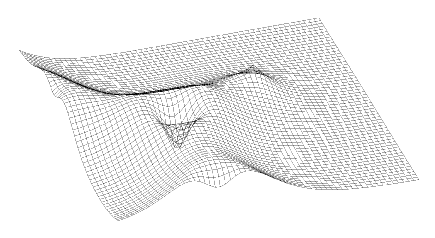
\includegraphics{benzene} \\~\\
\begin{latexonly}
\parbox{30em}{Keywords used:

\comp{MULT=1 CENTER=(-0.27,-0.5,0) LINE=(0,0,1) EDGE=3 AXIS=.4 GRID NO-CONTOURS}

This type of plot is best viewed with the contours added in, but for the
sake of clarity they have been omitted from this picture.}
\end{latexonly}
\begin{htmlonly}
Keywords used:

\comp{MULT=1 CENTER=(-0.27,-0.5,0) LINE=(0,0,1) EDGE=3 AXIS=.4 GRID NO-CONTOURS}

This type of plot is best viewed with the contours added in, but for the
sake of clarity they have been omitted from this picture.
\end{htmlonly}
\end{center}
\caption{Detail of C-H bond in benzene}
\end{figure}

% 21 lines, including this one
% \setlength{\unitlength}{0.06cm}
\begin{figure}
\begin{makeimage}
\end{makeimage}
\index{Polyacetylene!DENSITY plot}
\index{Graphite!DENSITY plot}
\begin{center}
\includegraphics{polyacetylene_total} \\~\\
\begin{latexonly}
\parbox{30em}{Keywords used are:

\comp{CENTER=(0.0,0.0,0.0) LINE=(0,0,1) EDGE=7.0}

The picture is centered on atom C$_1$, and shows the `join' of the central
unit cell with the adjacent unit cell.  Note that the `join' is quite
invisible.}
\end{latexonly}
\begin{htmlonly}
Keywords used are:

\comp{CENTER=(0.0,0.0,0.0) LINE=(0,0,1) EDGE=7.0}

The picture is centered on atom C$_1$, and shows the `join' of the central
unit cell with the adjacent unit cell.  Note that the `join' is quite
invisible.
\end{htmlonly}
\end{center}
\caption{\label{d_solids}Total electron density map for polyacetylene}
\end{figure}

\begin{figure}
\begin{makeimage}
\end{makeimage}
\begin{center}
\includegraphics{polyacetylene_pi} \\~\\
\begin{latexonly}
\parbox{30em}{Keywords used:

\comp{CENTER=(0.0,0.0,0.6) LINE=(0,0,1) EDGE=7.0 BONDS}

As with benzene, note the build-up of density {\em between} all
bonded pairs of atoms.  In order to show the strong $\pi$-bond, the
center of the plot has been raised 0.6\AA\ above the backbone chain.}
\end{latexonly}
\begin{htmlonly}
Keywords used:

\comp{CENTER=(0.0,0.0,0.6) LINE=(0,0,1) EDGE=7.0 BONDS}

As with benzene, note the build-up of density {\em between} all
bonded pairs of atoms.  In order to show the strong $\pi$-bond, the
center of the plot has been raised 0.6\AA\ above the backbone chain.
\end{htmlonly}
\end{center}
\caption{\label{d_solids1}Bonds map for polyacetylene}
\end{figure}

\begin{figure}
\begin{makeimage}
\end{makeimage}
\begin{center}
\includegraphics{graphite001} \\~\\
\begin{latexonly}
\parbox{30em}{Keywords used:

\comp{CENTER=(0.0,0.0,0.0) LINE=(0,0,1) EDGE=4.0}

The center of the plot is at C$_{1,1}$ in a 5 $\times$ 5 array of atoms.
The picture therefore shows the `join' of four unit cells, cells (0,0),
(0,-1), (-1,0), and (-1,-1).  As with polyacetylene, the `join' is
invisible.}
\end{latexonly}
\begin{htmlonly}
Keywords used:

\comp{CENTER=(0.0,0.0,0.0) LINE=(0,0,1) EDGE=4.0}

The center of the plot is at C$_{1,1}$ in a 5 $\times$ 5 array of atoms.
The picture therefore shows the `join' of four unit cells, cells (0,0),
(0,-1), (-1,0), and (-1,-1).  As with polyacetylene, the `join' is
invisible.
\end{htmlonly}
\end{center}
\caption{\label{d_solids2}Graphite, Total Electron Density}
\end{figure}

The program DENSITY is designed to generate  maps of electron density
distribution and molecular orbital intensity within molecules
(Figure~\ref{d_mol}) and solids (Figure~\ref{d_solids}). Two main modes of
operation are provided: manual data input, which is a ``stand-alone'' mode, and
normal input, which assumes the existence of large unformatted data-files
produced  by, e.g.\ MOPAC.

\index{GRAPH!use in DENSITY} To generate the large unformatted data-file, MOPAC
should be run using the key-word \comp{GRAPH}. At present, MOPAC can only
produce graphics files in the RHF mode, the UHF capability having not yet being
written.

Although DENSITY has a very simple data-input, users are warned that care is
needed in precisely wording a request. As an example, in learning how to use
DENSITY a user might want to plot the highest-filled $\pi$ orbital in benzene,
and choose the plane to be that of the carbon atoms. At first sight this
appears reasonable, but when one recalls that the $\pi$ system has a node in
this plane, another choice of plane is seen to be essential. A better choice of
plane would be one parallel to the plane of the carbon  atoms, but 0.5 to 1.0
\AA ngstroms above it.

Similarly, if only a detail of the molecule is to be studied, it is wasteful to
plot the whole molecule. The picture is essentially made up of 2,500 pixels, so
fine detail can very easily be lost if the whole molecule is used.

With one important exception the whole program is written using the FORTRAN-77
standard, so translation to allow DENSITY to run on different machines should
not be difficult. FORTRAN-77 does not support graphical functions, and an
interface, designed to allow users to easily write their own interfaces, has
been written.  This interface is, of course, machine-dependent.

\section{Data}
Rather than fully define the input, a worked example will be given
(Figure~\ref{d_c2h4}) and other data-files can then be generated by analogy.

\subsection{Example of Data: Ethylene}
\index{Ethylene! $\pi$-density in}
For this example we will use the $\pi$ system in ethylene. Two pictures are to
be drawn based on the results from an earlier MOPAC calculation.  The first
plot is in the plane parallel  to the plane of the molecule, the second one is
in the plane perpendicular to the C-C axis.  DENSITY data-files should have the
suffix \comp{.gra}.
\begin{figure}
\begin{makeimage}
\end{makeimage}
\begin{verbatim}
Line 1 :  DEBUG
Line 2 :  Ethylene pi system
Line 3a:  CENTER=(0.7,0.0,0.5) LINE=(0.0,0.0,1.0) EDGE=2.0 HOMO
Line 3b:  CENTER=(0.7,0.0,0.5) LINE=2 EDGE=2.0 HOMO
Line 4 :
\end{verbatim}
\caption{\label{d_c2h4} DENSITY data-set for Ethylene}
\end{figure}

\begin{description}
\item[Line 1:] First set of key-words.  These  control the mode of operation.
\item[Line 2:] Title of plot. Up to 79 characters can be used.
\item[Line 3a:] Second set of key-words. A full list of key-words, and
their definitions, is given in the next Section.
\item[Line 3b:] Key-words for the second picture.
\item[Line 4:] End the input with a blank line.
\end{description}

\subsection{Keywords}
Two sets of key-words are provided. At the start of a run the user must provide
information about the source of the molecular data. At present, this data can
come from one of two sources. These are (a) off the data-file itself, which is
the \comp{MANUAL} mode, and (b) from a disk or restart-type file, which was
created by an earlier run using MOPAC.

\subsection{Definitions of First set of Key-Words}
\begin{description}
\item[\comp{DEBUG}] Print part of working of DENSITY.
\item[\comp{DMAT}] Lower half triangle of density matrix to be read in (Used
with \comp{MANUAL} only)
\item[\comp{MANUAL}] Stand-alone  mode. All data supplied from datafile.
\item[\comp{M.O.}] A molecular orbital to be used as source of density matrix.
(Used with \comp{MANUAL} only)
\end{description}

\subsubsection*{\comp{DEBUG}}\index{DEBUG!use in DENSITY}
The density matrix or molecular orbital used by the density calculation will be
printed if \comp{DEBUG} is specified.

\subsubsection*{\comp{DMAT}}
To be used only if \comp{MANUAL} is also specified. \comp{DMAT} specifies that
the lower-half of the density matrix, in free-format, is read in. There would
be (NORBS$\times$(NORBS+1))/2 of these numbers.

\subsubsection*{\comp{MANUAL}}\index{MANUAL}
This word was used in the writing and de-bugging of DENSITY,  but now is only
intended for testing and demonstration purposes.

When \comp{MANUAL} is specified, either \comp{DMAT} or \comp{M.O.} must be
specified on the same line as \comp{MANUAL}.

If \comp{MANUAL} is specified, the following data must be supplied on the next
few lines:
\begin{enumerate}
\item Number of atoms, orbitals, and electrons (NATOMS, NORBS, NELECS).
One line, free format, integer.
\item Cartesian coordinates for each atom, one atom per line, free format,
real, in order x, y, z. There will be NATOMS of these.
\item Labels for all atoms. For example, all carbon atoms might be called
``1'', all hydrogen atoms ``2'', etc. Free format, integer. There will be NATOMS
of these numbers. The numbers must be 1 to NUNI, NUNI being the number
of unique atom-types in the molecule.

\begin{tabular}{llc|llllll|l} \hline
   Compound   &   Atom Labels       &NUNI &  \multicolumn{6}{c}{Line would read} & \\ \hline
  Methane     & C: 1,   H: 2        & 2 & 1 & 2 & 2 & 2 & 2 &       &   CH4  \\
  Formic Acid & H: 1,   C: 2,  O: 3 & 3 & 1 & 2 & 3 & 3 & 1 &        &  HCOOH  \\
  Thiomethanol& C: 1,   H: 2,  S: 3 & 3 & 1 & 2 & 2 & 2 & 3 & 2     &   CH3SH  \\ \hline
\end{tabular}

\item Atomic Numbers for all unique atoms. Free format, integer. There are
NUNI of these numbers. If atom of type 1 is a carbon atom, then the
corresponding atomic number would be 6. Using the examples above, we have:

\begin{tabular}{ll|lll} \hline
&                 Atomic Numbers & \multicolumn{3}{c}{Line would read}  \\
     Compound     &  Unique atom: &  1 &  2 &  \ 3 \\\hline
     Methane      &          &       6  & 1 & \\
     Formic Acid  &           &      1  & 6 & \  8 \\
     Thiomethanol &           &      6  & 1 & 16 \\ \hline
\end{tabular}

\item Principal Quantum numbers. Free format, integer. There are
NUNI of these numbers.

\begin{tabular}{ll|lll}
\hline
  & Principal Quantum Numbers  & \multicolumn{3}{c}{Line would read}  \\
     Compound &  Unique atom: & 1 & 2 & 3
\\ \hline
     Methane  &               & 2 & 1 &    \\
     Formic Acid  &           & 1 & 2 & 2    \\
     Thiomethanol &           & 1 & 2 & 3    \\
\end{tabular}

\item Number of orbitals for all unique atoms. Free format, integer, there are
NUNI of these numbers.

\begin{tabular}{ll|lll}
\hline
&            Number of Orbitals  & \multicolumn{3}{c}{Line would read} \\
     Compound &  Unique atom: & 1 & 2 & 3  \\
               \hline
     Methane  &                4 & 1  \\
     Formic Acid  &            1 & 4 & 4  \\
     Thiomethanol &            1 & 4 & 9  \\
\hline
\end{tabular}

\item Orbital exponents for all unique atoms, format is 3F10, three numbers
per atom (one each for $s$, $p$, and $d$ orbital exponents); if $p$ or $d$ is
absent, these can be left blank.

\begin{tabular}{lc|lll} \hline
 Compound & Unique atom &  \multicolumn{3}{c}{Line would read} \\ \hline
     Methane       &      1      & 1.78  &    1.78  \\
                   &      2      & 1.3&  \\
     Thiomethanol  &      1      & 1.78  &    1.78  \\
                   &      2      & 1.&  \\
                   &      3      & 2.4   &    2.1   &    1.0  \\ \hline
\end{tabular}

\item If M.O.\  is specified, the eigenvector coefficients are read in
at this point. Free format, there
are NORBS of these. Otherwise, if DMAT specified, the lower-half
of the density matrix, in free-format, is read in. There would be
(NORBS$\times$(NORBS+1))/2 of these numbers.
\end{enumerate}

\begin{figure}
\begin{makeimage}
\end{makeimage}
\compresstable
\begin{verbatim}
Line  1:      MANUAL       M.O.                   (Key-words
Line  2:      FORMIC ACID                         (Title
Line  3:      5  14 18                            (NATOMS, NORBS, NELECS
Line  4:   0.0000    0.0000    0.0000             (Cartesian coordinates
Line  5:   1.2270    0.0000    0.0000
Line  6:   1.9164    1.1676    0.0000
Line  7:   1.3973    1.9625    0.0000
Line  8:   1.8882   -0.8836    0.0000
Line  9:    1 2 1 3 3                             (Labels
Line 10:    8 6 1                                 (Atomic Numbers
Line 11:    2 2 1                                 (Princ. Quant. Nos.
Line 12:    4 4 1                                 (Orbitals per atom
Line 13:   2.699905  2.699905                     (Exponents
Line 14:   1.787537  1.787537
Line 15:   1.331967                    (below: eigenvector coefficients
Line 16:   -0.1616  0.4769  -0.0514   0.0000  -0.0628  -0.3488  -0.0032
Line 17:    0.0000  0.2634   0.6282  -0.0893   0.0000  -0.2925  -0.2457
Line 18:    CENTER=2 LINE=(0,0,1) EDGE=4          (Rest of data
\end{verbatim}
\caption{\label{d_hcooh} Full Example of Manual Data for Formic Acid}
\end{figure}

\subsubsection*{\comp{M.O.}}
This keyword is to be used only when \comp{MANUAL} is also specified. A
molecular orbital to be used as source of density matrix.  The M.O.\ comes
after the other data required by \comp{MANUAL} as a set of free-format
coefficients. After all these data are read in, the program continues as usual,
but many limitations apply. For example, if \comp{M.O.} was used, then the
key-words  \comp{PSI=$n$}, \comp{HOMO} and \comp{LUMO} would all give the same
result. These limitations are due to the absence of other data. The second set
of key-words defines the type of plot to be drawn; much of this data is
obligatory in that there are no defaults for certain data. The user must
supply:
\begin{itemize}
\item A definition of the center of the plot.
\item A definition for the axis of the vector perpendicular to the plot.
\item A length, in \AA ngstroms, of the edge of the plot.
\end{itemize}
Other data, which are mutually exclusive, are:
\begin{itemize}
\item A molecular orbital number, given by \comp{PSI=$n$}, or
\item A highest-occupied molecular orbital, defined by the key-word
 \comp{HOMO}, or
\item A lowest-unoccupied molecular orbital, defined by the
key-word \comp{LUMO}, or
\item The explicit molecular-orbital occupancy, see key-word \comp{OCCUPANCY}, or
\item The normal electron density of the molecule. This is specified by
the absence of the other key-words; i.e., this is the default.
\end{itemize}
If a full electron density map is specified. (That is, if the last option
above is taken), then another key-word, \comp{BONDS}, can be used. \comp{BONDS}
will remove the electron density due to the atom from the plot. The effect of
this is to  generate a plot showing where the charge build-up in the bonds
occurs. Note: Ionic separations are not shown by \comp{BONDS}.

\subsection{Definitions of Second set of Key-Words}
\begin{description}
\item[\comp{ADD}] The current plot is to be added to the next plot.
\item[\comp{AXIS=$n.nn$}] Angle of plane of plotted square to viewer's eye.
\item[\comp{BONDS}] Subtract the electron density due to the atoms.
\item[\comp{CENTER}] Used to define the center of the plot.
\item[\comp{EDGE=$n.nn$}] Definition of the length of one side of the plot.
\item[\comp{FINE}] Produce four times the default number of contours.
\item[\comp{GRID}] Overlay x-y grid onto plot. Used with AXIS.
\item[\comp{HOMO}] Plot the highest occupied M.O.
\item[\comp{LINE}] Used to define the axis perpendicular to the plot.
\item[\comp{LUMO}] Plot the lowest unoccupied M.O.
\item[\comp{MULT=$n.nn$}] Multiply vertical relief by specified amount.
\item[\comp{OCCUPANCY}] Used to allow the individual M.O.\ populations to be specified.
\item[\comp{PSI=$n$}] Plot a specific M.O.
\item[\comp{PHASE}] Multiply the current plot by a constant.
\end{description}

\subsubsection*{\comp{ADD}\index{ADD}}
When two or more pictures are to be added together to form a single picture,
\comp{ADD} must be used. For example, a user might want to add or subtract
two M.O.s to see the effect. Thus if M.O.\ 2 and M.O.\ 3 were to be
added together, the data for such a calculation could be:
\begin{verbatim}
Line 1:
Line 2:   FORMALDEHYDE
Line 3: CENTER=2 LINE=(0,0,1) EDGE=2 PSI=2 ADD
Line 4: CENTER=2 LINE=(0,0,1) EDGE=2 PSI=3
Line 5:
\end{verbatim}
See also \comp{PHASE}.

\subsubsection*{\comp{AXIS=$n.nn$}\index{AXIS}}
A square plot is drawn by default. If the user wants to show the
three-dimensional nature of the contour map a facility exists to tilt the plot
so that a foreshortened and rotated plot is drawn. Of course, the degree of
tilt depends very much on the system; there is no facility in DENSITY to
eliminate ``hidden lines'', so the tilt should not be so great that hidden
lines would show. The range of $n.nn$ in  \comp{AXIS=$n.nn$} is 1.0 to 0.0. 1.0
(the default) would give a square plot, as if the user was viewing the plot
from directly overhead looking straight down; 0.0 gives a view of the plot as
if the user was looking at it from the horizon, looking horizontally. Clearly,
\comp{AXIS=1.0} would not show the relief. If \comp{GRID} were used only a
perfectly featureless square grid would be seen. Conversely, \comp{AXIS=0.0}
would show the contours as perfectly flat, straight lines. Therefore, a better
choice would be \comp{AXIS=0.6}.

\subsubsection*{\comp{BONDS}\index{BONDS!use in DENSITY}}
Not to be used in conjunction with \comp{HOMO}, \comp{LUMO},
\comp{PSI=$n$}, or \comp{OCCUPANCY}.
\comp{BONDS} calculates the average atomic orbital occupancy of each atom,  and
subtracts that number from the density matrix. The result is a plot whose
average value is zero, and which shows where the electrons have come from and
gone to when the bonds are formed.

\subsubsection*{\comp{CENTER}\index{CENTER}}
This key-word is essential. It defines the center of the plot (see
Section~\ref{area}). Two formats are provided to define the center: (a) an atom
number can be used, and (b) an absolute Cartesian coordinate  can be specified.

\begin{description}
\item[Definition by atom number]~\\
Format: \comp{CENTER=$n$}  The location of atom $n$ is defined as the center
of  the plot. Thus if atom $n$ has Cartesian coordinates (x=0.5, y=1.4, z=-0.8)
then the center of the plot is (x=0.5, y=1.4, z=-0.8). Dummy atoms are not
counted, so if any dummy atoms were used in the definition of the geometry,
they must be ignored when considering the atom number. In other words, only a
real atom can be used to define a point in the molecule.

\item[Definition by absolute Cartesian coordinate]~\\
Format: \comp{CENTER=($n.nn$,$n.nn$,$n.nn$)} The location of the  center of the
plot is defined as ($n.nn$,$n.nn$,$n.nn$). Of course, before such a center can
be defined, the user must know the Cartesian coordinates of the atoms in the
molecule.
\end{description}

Regardless of which option is used, the center of the plot will be converted
internally into absolute Cartesian coordinates.

\subsubsection*{\comp{FINE}}
Normally, between 10 and 25 contours are plotted. In order to increase this
number, \comp{FINE} can be used, in which case 40 to 100 contours will be
generated.

\subsubsection*{\comp{EDGE=$n.nn$}\index{EDGE}}
The length of one side of the graph-plot is defined as being $n.nn$  \AA ngstroms.

\subsubsection*{\comp{GRID}\index{GRID!use in DENSITY}}
\comp{GRID} can be used to enhance the legibility of a plot. It draws a regular
mesh of lines across the plot, with the same relief as the contours.
\comp{GRID} should only be used with an \comp{AXIS} which is not 1.0.

\subsubsection*{\comp{HOMO}\index{HOMO!use in DENSITY}}
For closed-shell systems with non-degenerate highest occupied molecular
orbitals, the key-word \comp{HOMO} can be used to produce an intensity map of
the highest occupied molecular orbital. For other systems, the key-word
\comp{PSI=$n$} should be used.

\subsubsection*{\comp{LINE}\index{LINE}}
This key-word is essential. It defines the vector perpendicular to the plane
of the plot, see Section~\ref{area}. Two formats are provided to define the axis
perpendicular to the plane of the plot; these formats use radically different
concepts, so users are cautioned to verify that they understand both
definitions and the distinction between them.
(a) an atom number can be used, and (b) an absolute Cartesian coordinate
can be specified.

\begin{description}
\item[Definition by atom number]~\\
Format: \comp{LINE=$n$}  The axis of the plot is defined  by the vector drawn
from  atom $n$ to the defined center of the plot. Thus if atom $n$ has
Cartesian coordinates (x=0.5, y=1.4, z=0.2) and the center of the plot is at
point (x=0.5, y=1.4, z=-0.8) then the axis of the plot is (0.0, 0.0, 1.0).
Dummy atoms are not counted, so if any dummy atoms were used in the definition
of the geometry, they must be ignored when considering the atom number. In
other words, only a real atom can be used to define the axis of the graph.

\item[Definition by absolute Cartesian coordinate]~\\
The vector need not be  normalized, but must not be of zero length.

Format: \comp{LINE=($n.nn$,$n.nn$,$n.nn$)} The axis of a  line perpendicular to
the plane of the plot is ($n.nn$,$n.nn$,$n.nn$). This axis need not be
normalized, but must be finite; that is, the only axis not allowed is (0,0,0).
\end{description}

Irrespective of which option is used, the axis of the plot will be converted
internally into a unit vector in Cartesian coordinates.

\subsubsection*{\comp{LUMO}\index{LUMO!use in DENSITY}}
For closed-shell systems with non-degenerate lowest unoccupied molecular
orbitals, the key-word \comp{LUMO} can be used to produce an intensity map of
the lowest unoccupied molecular orbital. For other systems, the key-word
\comp{PSI=$n$} should be used.

\subsubsection*{\comp{MULT=$n.nn$}\index{MULT}}
There is a default scale for the relief of a plot, when viewed as a 3-D
structure. If this default is not suitable, say the plot is too flat, then
\comp{MULT=$n.nn$} can be used to change the vertical scale.  \comp{MULT=1.0}
will do nothing, \comp{MULT=2.0} will increase the vertical relief.

\subsubsection*{\comp{OCCUPANCY}\index{OCCUPANCY}}
When the user wants to explicitly define an electronic configuration for a
system, \comp{OCCUPANCY} is used. This key-word requires the explicit occupancy
of the M.O.s to be defined on the next line, in I1 format. For example, to
define methane with one electron in each of the three triply-degenerate levels,
the lines
\begin{verbatim}
Line 1:CENTER=1 LINE=(0.0,0.0,1.0) OCCUPANCY EDGE=2.0
Line 2:2111
\end{verbatim}
could be used. Similarly, if an excited ethoxy radical were to be specified,
the following definition could be used:
\begin{verbatim}
Line 1:CENTER=(0.7,0.0,0.0) LINE=(0.0,0.0,1.0) OCCUPANCY EDGE=2.0
Line 2:22222201
\end{verbatim}

\subsubsection*{\comp{PHASE}\index{PHASE}}
Two formats for this are possible. If \comp{PHASE} is specified, the data being
added to the plot is multiplied by -1, i.e.\ negated.  If \comp{PHASE=$n.nnnn$}
is used, the data are multiplied by $n.nnnn$. For example, to form the
normalized M.O.\ of formaldehyde resulting from equal and opposite amounts of
the second and third M.O.s, i.e.\ 0.7071(M.O.2 $-$ M.O.3), the following  data
could be used.
\begin{verbatim}
Line 1:
Line 2:   FORMALDEHYDE
Line 3: CENTER=2 LINE=(0,0,1) EDGE=1 PSI=2 PHASE=0.7071 ADD
Line 4: CENTER=2 LINE=(0,0,1) EDGE=1 PSI=3 PHASE=-0.7071
Line 5:
\end{verbatim}
Note that the first phase is positive. It is not the plot that is reversed,
only the data going in to the plot, so that the data arising from line 4 are to
be multiplied by -0.7071 before being added to the plot.

\subsubsection*{\comp{PSI=$n$}}
A specified molecular orbital is to be plotted. Note that degenerate M.O.s
cannot be unambiguously represented, as they are ill-defined by a random
unitary transform. To plot degenerate M.O.s the user should be prepared to use
\comp{PHASE} and \comp{ADD}.

\subsection{Calculation of Excited State Density}
Excited states can be represented by a linear combination of Slater
determinants.  As far as electron density is concerned, each determinant, or
{\em microstate}, can be represented by a set of molecular orbital occupancies,
without regard for spin.  By use of \comp{OCCUPANCY}, any spin-free microstate
can be defined.  These facts can be used in the calculation of state densities.

State densities can be calculated by adding together the densities arising from
various microstates, weighted by their contribution to the overall state.
The weight is given simply by the square of the coefficient of the microstate
in the state.

As an example, consider the state density arising from the fourth state in
formaldehyde.  Keywords used in MOPAC would be:\\ \comp{LARGE MECI PRECISE
GRADIENTS C.I.=2  ROOT=4 GRAPH} \\ and the microstates used in the MECI
calculation are shown in Figure~\ref{fourth}. In this system, the HOMO is
molecular orbital 6, and the LUMO is molecular orbital 7.

\begin{figure}
\begin{makeimage}
\end{makeimage}
\begin{center}
%    ()(n1,n2) n1 = start horizontal, distance left
%              n2 = start vertical, distance down
%  -4,2 = 4 inches in and 2 inches down
\setlength{\unitlength}{1in}
\begin{picture}(6.0,1.2)(0.0,0.0)
\put(1.2,1.2){Microstate 1}
\put(2.2,1.2){Microstate 2}
\put(3.2,1.2){Microstate 3}
\put(4.2,1.2){Microstate 4}
\put(0.8,0.65){LUMO}
\put(0.8,0.05){HOMO}
\put(2.5,0.1){\line(1,0){0.2}}
\put(2.5,0.7){\line(1,0){0.2}}
\put(2.55,0.68){$\downarrow$}
\put(2.55,0.08){$\uparrow$}
\put(3.5,0.1){\line(1,0){0.2}}
\put(3.5,0.7){\line(1,0){0.2}}
\put(3.55,0.68){$\uparrow$}
\put(3.55,0.08){$\downarrow$}
\put(1.5,0.1){\line(1,0){0.2}}
\put(1.5,0.7){\line(1,0){0.2}}
\put(1.53,0.08){$\uparrow$}
\put(1.60,0.08){$\downarrow$}
\put(4.5,0.1){\line(1,0){0.2}}
\put(4.5,0.7){\line(1,0){0.2}}
\put(4.53,0.68){$\uparrow$}
\put(4.60,0.68){$\downarrow$}
\end{picture}

\end{center}
\caption{\label{fourth}Configurations used with C.I.=2}
\end{figure}

The linear combinations of microstates in the state functions are given in the
output, as shown in Figure~\ref{ci_output}.

\begin{figure}
\begin{makeimage}
\end{makeimage}
\begin{verbatim}
   Root No.    1       2       3       4

              1 A1    1 A2    2 A2    2 A1

               0.0     2.5     2.9     7.5

         1  0.9997  0.0000  0.0000  0.0256
         2  0.0000  0.7071 -0.7071  0.0000
         3  0.0000  0.7071  0.7071  0.0000
         4 -0.0256  0.0000  0.0000  0.9997
\end{verbatim}
\caption{\label{ci_output}State functions in Formaldehyde arising from C.I.=2}
\end{figure}

The electron density contour map for the fourth state can be generated by use
of \comp{OCCUPANCY}, \comp{ADD}, and \comp{MULT}, thus:
\compresstable
\begin{verbatim}
   Formaldehyde, Electron Density for the fourth state
CENTER=(0.7,0.0,0.1) LINE=(0.0,0.0,1.0) EDGE=3.0 OCCUPANCY PHASE=0.000655 add
2222220
CENTER=(0.7,0.0,0.1) LINE=(0.0,0.0,1.0) EDGE=3.0 OCCUPANCY PHASE=0.999400
2222202
\end{verbatim}
\normalsize
The corresponding data set for DENSITY for the third state would be:
\compresstable
\begin{verbatim}
   Formaldehyde, Electron Density for the third state
CENTER=(0.7,0.0,0.1) LINE=(0.0,0.0,1.0) EDGE=3.0 OCCUPANCY PHASE=0.500000 add
2222211
CENTER=(0.7,0.0,0.1) LINE=(0.0,0.0,1.0) EDGE=3.0 OCCUPANCY PHASE=0.500000
2222211
\end{verbatim}
\normalsize
However, because the electron density arising from microstates 2 and 3 is the
same, this data set could be written in a more compact form, thus:
\compresstable
\begin{verbatim}
   Formaldehyde, Electron Density for the third State
CENTER=(0.7,0.0,0.1) LINE=(0.0,0.0,1.0) EDGE=3.0 OCCUPANCY
2222211
\end{verbatim}
\normalsize
Finally, note that the electron density distribution for the second and third
states are the same.  With \comp{C.I.=2}, the first excited state, a triplet,
and the second excited state, the first excited singlet, have the same electron
density everywhere.

\subsection{Definition of the area of the graph plot}\label{area}
The graph plot is a square, which represents a slice or cut through the volume
of a molecule. To define a square, seven numbers are needed. In order, these
are:
\begin{itemize}
\item Three numbers to define the position of the center of the square.
\item Three numbers to define an axis perpendicular to the surface of the square.
\item One number to define the length of the edge of the square.
\end{itemize}
To specify the center of the square, the key-word \comp{CENTER} is  provided.
\comp{CENTER} can be either an atom number, e.g.\ \comp{CENTER=4}, or an
absolute Cartesian  coordinate, e.g.\ \comp{CENTER=(0.6,0.5,2.4)}. If an atom
is used, the absolute Cartesian coordinates of that atom are used to define the
center of the square. In either case, the center of the square, i.e.\ the
intersection of the two diagonals of the square, is defined by the resulting
absolute Cartesian coordinate.

Examples:
\begin{itemize}
\item Methane, center of plot to be on one of the hydrogen atoms, these
being atoms 1, 3, 4, and 5. Use \comp{CENTER=1} or \comp{CENTER=3} etc.; as an
alternative, assuming the first atom is at the origin,
\comp{CENTER=(0.0,0.0,0.0)} could be used.
\item Benzene, given Cartesian coordinates as follows:
\begin{verbatim}
             X         Y         Z
  C1       0.0000    0.0000    0.0000
  C2       1.4066    0.0000    0.0000
  C3       2.1099    1.2182    0.0000
  C4       1.4066    2.4363    0.0000
  C5       0.0000    2.4363    0.0000
  C6      -0.7033    1.2182    0.0000
  H1      -0.5451   -0.9442    0.0000
  H2      -0.5451    3.3805    0.0000
  H3       1.9517   -0.9442    0.0000
  H4      -1.7935    1.2182    0.0000
  H5       3.2002    1.2182    0.0000
  H6       1.9517    3.3805    0.0000
\end{verbatim}
Then, if a plot of benzene with the center of the molecule at the middle
of the picture, \comp{CENTER=(0.7,1.2,0.0)} could be used.
\item Benzene, $\pi$-system. Using the above Cartesian coordinates for the
benzene ring, the center of the plot must be above the plane of the
ring in order to avoid the nodes in the $\pi$-system. In this case
\comp{CENTER=(0.7,1.2,0.5)} would be appropriate.
\end{itemize}
 Once the center of the plot is defined, the orientation of the plane
of the plot needs to be specified. Thus if a plot of methane was wanted,
and the center of the plot was on the carbon atom, the following
cross-sections could be drawn:
\begin{itemize}
\item Four-fold symmetry: Plot is oriented in the reflection plane of the
S$_4$ symmetry operation. To specify this, absolute Cartesian
coordinates would need to be used.
\item Three-fold symmetry: Axis of plot is from carbon to any hydrogen.
To specify this, \comp{LINE=4} could be used.
\item Showing two C-H bonds: Given that the first three atoms are H, C, and
H, then the axis (0.0,0.0,1.0) would be perpendicular to the plane
of  these three atoms (assuming that all three atoms had the same z component).
\end{itemize}
 It might be helpful in visualizing the axis of the plot by imagining the plot
without the line specified. The center of the plot is already defined, but
the square is still free to rotate in all three dimensions, so only one
point in the square is defined. The plane of the plot is then
defined by \comp{LINE}.

The final unknown is the size of the plot. This is
specified by \comp{EDGE=$n.nn$}.
The length $n.nn$ defines the length, in \AA ngstroms, of the side of the plot.
Note that most molecules are bigger than their simple atomic coordinates
would suggest. As an example, to get a benzene ring to fit inside a plot,
\comp{EDGE=6.0} would be needed, even though the H-H distance across the ring is
only 4.8-5.0 \AA ngstroms.
\section{Details of Graph Plots}
\subsection{Contours}\index{Contours}
 There are normally between 10 and 25 contours. The contours are separated
by steps of size 1, 2.5, and 5 times 10 to some integer power. The most
common step sizes are:
\begin{verbatim}
 0.0010, 0.0025, 0.0050, 0.0100, 0.0250, 0.0500,
 0.1000, 0.2500, 0.5000, 1.0000, 2.5000, 5.0000
\end{verbatim}
in units of electrons per cubic \AA ngstrom, for electron density, and
the square root of these units for wave-functions.

 The flexible nature of the step size means that the user can expect to see
something in the picture, but close attention should be paid to the contour
interval. If the step size is excessively small, less than 0.00001,
the user will be warned, but the calculation will be continued.

\subsection{Density Around Atoms}
 All Slater atomic orbitals have a node at the nucleus, with the
important exception
of hydrogen. One result of this is that hydrogen is the only element whose
electron density has a maximum at the nucleus. All other atoms have an almost
zero electron density at their nucleus. This is usually disconcerting
at first sight,
but is a consequence of the behavior of Slater-type orbitals.
 For planar systems, it is a good idea to plot the density in the plane
a fraction of an \AA ngstrom above the plane of the molecule.
\subsection{Difference Maps}\index{Difference maps}
 A difference map shows where electron density builds up when bonds are
formed. It will NOT show ionic character. To form a \comp{BONDS} map
the electron density arising from the atoms is spherically averaged and
then subtracted from the density matrix. For example, suppose the atomic
orbital populations on an atom arising from the un-renormalized eigenvectors
are  1.0, 1.1, 1.2, and 1.3 for $s$, $p_x$, $p_y$, and $p_z$,
respectively. Then the
spherically averaged populations are 1.0, 1.2, 1.2, and 1.2 for these atomic
orbitals.
\subsection{Renormalization of Molecular Orbitals}
  All maps are calculated from data originally derived from the supplied
molecular orbitals. These M.O.s are presumed to be un-renormalized: that
is, the sum of the squares of the coefficients of the M.O.s add to unity.
The first step, therefore, is to re-normalize the M.O.s. This is done
by matrix multiplying the starting eigenvector matrix by the
inverse-square-root of the overlap matrix. This requires the presence of
the inverse-square-root of the overlap matrix, which must be supplied by
the MOPAC file. If re-normalization is not done, the total
electron density would be too large, and the difference maps would be
quite incorrect.


\section{Programming Considerations}
 DENSITY is not intended to be a ``stand-alone'' program. Its main purpose
is to be run using data generated by an earlier MOPAC calculation.
Results from DENSITY need some further processing before a hard-copy
graph-plot is obtained.
 In order, then, the unformatted data required from
a MOPAC type calculation to be used as auxiliary
data for DENSITY are as follows:

Record:

\begin{enumerate}
\item Number of Atoms, Number of Orbitals, Number of Electrons,
X-Cartesian coordinates for all atoms, Y-Cartesian coordinates for all atoms,
Z-Cartesian coordinates for all atoms.
\item Stopping and starting orbital counters for all atoms.
\item $s$-orbital exponents for all atoms, $p$-orbital exponents for all atoms,
$d$-orbital exponents for all atoms. Atomic numbers for all atoms.
\item All the un-renormalized eigenvectors, atomic orbital indices running
fastest.
\item Lower half triangle of the inverse-square-root of the overlap matrix.
\end{enumerate}
 DENSITY produces a default file suitable for a plotting program to use.
This file has the following format:

 Line 1: This line consists of the single, unchanging, message
\begin{verbatim}
                    NUMBER OF CONTOURS =  nn,
\end{verbatim}
with  $nn$  the actual number of different contours supplied. The programmer
can use this message to detect the start of a contouring file, and, if
desired, make use of the number nn to decide what action to take.

 Lines 2-4: Text. The programmer should print these lines without assuming
that the text makes any sense.

 Lines 5 on: The layout of these lines is as follows:
\begin{verbatim}
     <x-coordinate> <y-coordinate> <Pen code>  <Contour Height>
\end{verbatim}
As the whole plot is within the range 0.0 to 1.0, the x- and y-coordinates
are fractions of unity. The pen code is integer, 1 for pen up, 2 for pen down.
The contour height is real, and self-explanatory.

 Near to the end of the file is a single contour of height 99.999. This
 ``contour''
draws a box around the plot.

 Finally, the last few lines are the chemical symbols. These use the
same layout as Lines 5 on, but in place of the pen code, the chemical symbols
are present.
If this output is not
suitable, the programmer should modify subroutine PLOTGR.

\section{Description of Program}
\subsection{Fortran Files}
 DENSITY consists of several FORTRAN-77 files. These are:
\begin{description}
\item[CNTOUR] A general 2 or 3-dimensional contour-drawing subroutine.
\item[DRAW] A subroutine to draw one contour.
\item[EULER] Rotates a point in 3-D space.
\item[DATIN] Reads in data defining one particular picture.
\item[MAIN] Main segment; generates array for contouring.
\item[MAXMIN] Calculates highest and lowest points in the picture.
\item[PLOTGR] Interface between FORTRAN-77 and graphics routine.
\item[READIN] Gets in data defining molecule
\item[PLOTGR] Generates data for graph plotter.
\end{description}

\subsection{Description of FORTRAN Files}
\paragraph*{CNTOUR}\index{CNTOUR}
CNTOUR is a general contour-drawing routine. It calls subroutines
DRAW, EULER, and MAXMIN. The contour map can be tilted to show the
three-dimensional structure of the density map.

\paragraph*{DRAW}
 Draws a single contour, given a starting address. Called by CNTOUR
to allow users to rapidly write their own interfaces.

\paragraph*{EULER}\index{EULER}
 Performs a three-dimensional rotation on a three-dimensional
point provided; the resulting point is then used as a data
point for plotting.

\paragraph*{DATIN}
 All the user-supplied data defining a picture are read in in DATIN.
Some checking is done to ensure that the key-words provided are
compatible.

\paragraph*{MAIN}
 The main program, generates the wave-function in terms of atomic
orbitals, this is then used to calculate the pixel array, which in
turn is used by the contouring subroutine.

\paragraph*{MAXMIN}
 Prints the values and positions of the maxima and minima on the plot.
No data are altered by a call to MAXMIN.

\paragraph*{PLOTGR}\index{PLOTGR}
 The interface between FORTRAN-77 and the graphics routines is provided
by PLOTGR. Only very simple graphics commands are used, in order to
permit easy conversion of the program to run on other machines.
Programmers will need to change PLOTGR to suit local equipment.

\section{Installing Density}
DENSITY is distributed with MOPAC, and is normally written
to the sub-directories \comp{\ldots/density\_source/} and
\comp{\ldots/density\_examples}.

The parameter file SIZES should be read and, if necessary, modified before
\comp{Makefile} is run. The two parameters within SIZES that the user can
modify are MAXLIT and MAXHEV. MAXLIT is assigned a value equal to the largest
number of hydrogen atoms that a DENSITY job is expected to run, MAXHEV is
assigned the corresponding number of heavy (non-hydrogen) atoms.

Once you are satisfied with the contents of SIZES, compile DENSITY by issuing
the command `make'. Once this is complete, there is no  reason to keep the
object  files, and if space is at a premium these can be deleted at this time.
They should be kept if modifications are to be made to the program, in order to
allow rapid re-linking with the modified subroutines.

\section{Running DENSITY}
The command \comp{density} followed by a filename will start an on-line DENSITY
job.   E.g.\ \comp{density ethylene}, where \comp{ethylene.gra} is the data-set
for DENSITY, and a calculation of ethylene had been run earlier using MOPAC.

The main files that are required by DENSITY are:
\begin{center}
\begin{tabular}{ccl}
           File    &      Channel  &   Description \\ \hline
         \comp{$<$filename$>$.gpt}  &  13 &   MOPAC generated file. \\
         \comp{$<$filename$>$.gra}  &   5 &   User-generated data file \\
\end{tabular}
\end{center}
The main files that are produced are:
\begin{center}
\begin{tabular}{ccl}
           File     &    Channel &   Description  \\ \hline
        \comp{$<$filename$>$.out} &    6 &  Results  \\
        \comp{$<$filename$>$.tec} &   15 &  Formatted file of graph-plot \\
                                            for use by a graphics program. \\
\end{tabular}
\end{center}
